\documentclass{article}

\include{stddefs}
\include{imodefs}

\newcommand{\red}[1]{\textcolor{red}{\textbf{#1}}}
\newcommand{\green}[1]{\textcolor{green}{\textbf{#1}}}

\begin{document}

\chapterno{1}

\chapter{The language of mathematics}

We need to introduce some formal notation to be able to talk clearly about mathematics and also in a reasonable way 
formulate mathematical models of the real world. In modern mathematics the 
concept of a set is crucial. It is \url{a bit tricky}{https://en.wikipedia.org/wiki/Set_theory\#Axiomatic_set_theory} to define this precisely.
We will go on and define the basic concepts of what is called 
\url{naive set theory}{https://en.wikipedia.org/wiki/Naive_set_theory}.

\begin{frameit}
  \section{Black box warnings}

Modern mathematics is perhaps not like
anything you have encountered so far. It calls for a lot of focus and precision, especially when
writing down solutions to problems. It is a bit like programming a computer. There is no room for imprecision and half-baked sentences.

This course amounts to $10$ ECTS or approximately $280$ hours. Suppose that you spend
a week studying for the exam, say $40$ hours. Lectures, exercise classes and MatLab amount to $14\cdot (4 + 2 + 3)$ hours $= 126$ hours. This leaves around $114$ hours for your own study and immersion. Put in
other terms, you are supposed to work around $8$ hours per week outside classes for this course. With
classes, each week calls for $17$ hours of work. There is a very close relationship between the amount
of hours you log each week and your result at the exam. To state the obvious: numbers don't lie. If you
put in the time, you will almost certainly do well. Try to allocate time for IMO in your weekly
schedule and please (ab)use all the help that is provided. I am not saying that you should be as
disciplined as \url{Casey Neistat}{https://en.wikipedia.org/wiki/Casey_Neistat} or \url{Jocko Willink}{https://en.wikipedia.org/wiki/Jocko_Willink} (but you might learn something from them about organizing your time):

\youtube{C-Cvl3_CH2A}

Please note that you should shy away from the behavior indicated below, when you really want to focus on
learning. Be serious!

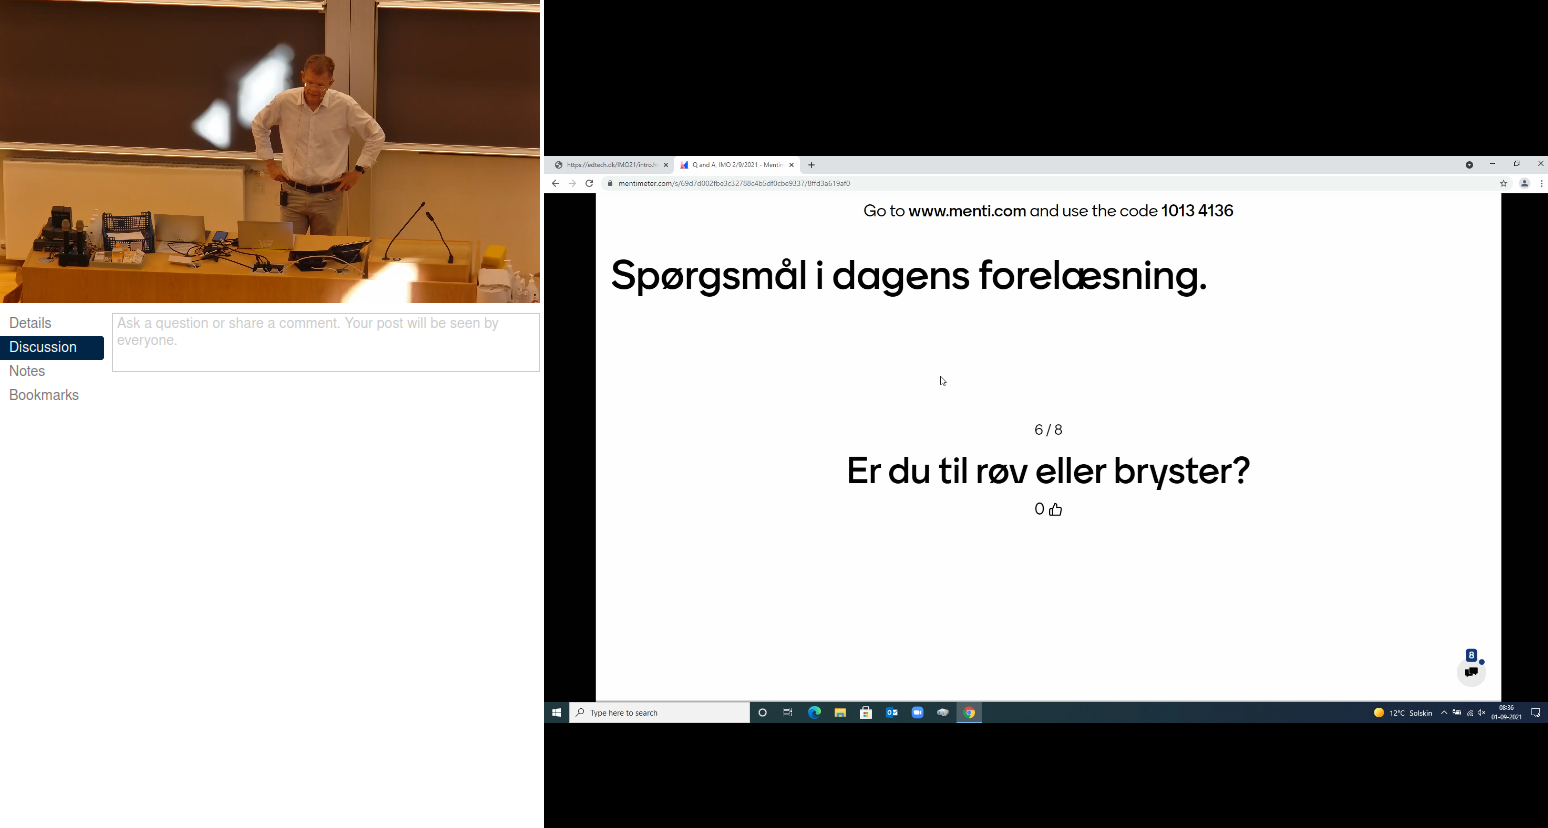
\includegraphics[width="75\%"]{spsmIMO.png}

Also, computers are exceptionally fun, but be careful! Nothing
really beats a clear thinking human mind. To wit, I asked \url{WolframAlpha}{https://wolframalpha.com} to solve a
certain optimization problem and it came up with the answer

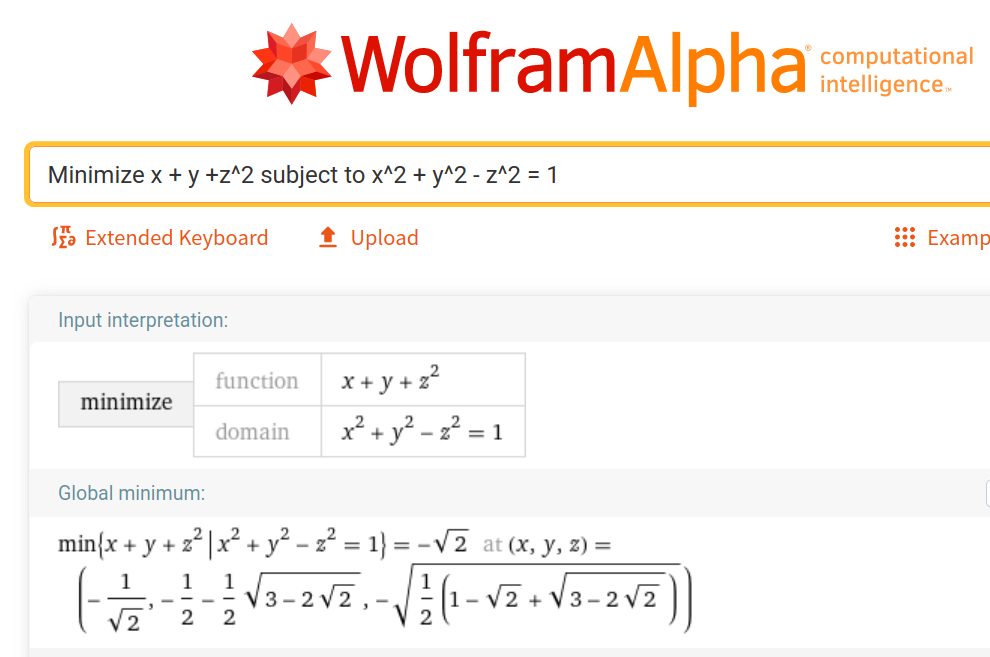
\includegraphics[width="75\%"]{WolframAlphaFails.png}

\beginshex
What is strange about this output?

\begin{hint}[showhide]
  Compute
  $$
  x = -\sqrt{\frac{1}{2} \left(1 - \sqrt{2} + \sqrt{3 - 2\sqrt{2}}\right)}
  $$
  on a pocket calculator (or similar) and see what you get using approximate decimal numbers.
  Explain your (stepwise) computation of $x$ using approximate decimal numbers.
  
  \begin{hint}[showhide]
  $$
  3 - 2 \sqrt{2} = (\sqrt{2} - 1)^2.
  $$
\end{hint}
\end{hint}
\endshex

\end{frameit}




\section{Computer algebra}

We will use the computer algebra system
\url{Sage}{https://www.sagemath.org/} in exploring and experimenting
with mathematics. This means that you will have to write small
commands and code snippets. Sage is built on top of the very wide
spread language
\url{Python}{https://en.wikipedia.org/wiki/Python_(programming_language)}
and you can in fact enter \footnote{Python code}{One may also enter code in several other languages, but I have so far only set the interface up for Sage and Python} in
the Sage input windows in this text. Below is an example of a basic
graphics command in Sage.  Push the Compute button to evaluate.


\begin{sage}
plot(sin(x) + cos(2*x), (x, 0, 2*pi))
\end{sage}

You can install Sage on your own computer following the instructions on
\url{https://www.sagemath.org/}{https://www.sagemath.org/}.

\beginshex
Did you notice that you can edit and enter new commands in the Sage window?
Do the following problems using Sage based on the \url{Sage guided tour}{http://doc.sagemath.org/html/en/tutorial/tour.html}. 

\begin{enumerate}[(i)]
\item Consider $f(x) = x \sin(1/x)$. Plot the graph of $f$ from $0$ to $0.1$. Computing $f(0)$ does not make sense. Do you
  see a way of assigning a natural value to $f(0)$ using the graph?
\item Find an approximate solution with four decimals to the equation $\cos(x) = x$.
  
  \begin{hint}[showhide]
    This is an example of an equation, that can only be solved numerically.
    Try first plotting the graph of $f(x) = x - \cos(x)$ from $0$ to $1$. Then use a
    suitable function from the Sage guide.
    \end{hint}
\item Compute $\pi$ with $100$ decimals.
\end{enumerate}
  
\endshex





\section{Objects or elements and the symbols $=$ and $\neq$}\label{eqobjects}

Mathematics can be broadly viewed as handling objects precisely
according to a specific system of rules. The first element
of precision is in distinguishing the objects and deciding when
they are the same. This calls for notation. If two objects
$x$ and $y$ are the same, we write $x = y$. If they are different
we write $x\neq y$.

You may laugh here, but identifying objects is really one of the fundamental tasks of mathematics.
It is not always that easy. Even though objects appear different they are the same as
in, for example
$$
\frac{105}{189} = \frac{35}{63}\qquad\text{and}\qquad \sin\left(\frac{\pi}{2}\right) = 1.
$$
The first example above is an identity of fractions (rational numbers). The second is
an identity, which calls for knowledge of the sine function and real numbers. Each of these
identities calls for some rather advanced mathematics.


\beginshex\label{sagecompex1}

\begin{sage}
var('a b')
e = (a+b)^2
e.expand()
\end{sage}

Use the Sage window above to reason 
about equality in the quiz below. In each case describe the objects i.e.,
are they numbers, symbols, etc.? Also, please check your computations
by hand with the old fashioned paper and pencil, especially $(a+b)(a-b)$.

\begin{quiz}
\question
Click on the right equalities below.
\answer{T}
$$a + b - 2 b = a - b$$
\answer{F}
$$(a+b)^2 = a^2 + b^2$$
\answer{T}
$$(a + b)(a - b) = a^2 - b^2$$
\answer{T}
$$(a + b)^2 = a^2 + 2 a b +  b^2$$
\answer{F}
$$(a+b)^3 = a^3 + 2 a^2 b + 2 a b^2 + b^3$$
\answer{F}
$$\frac{3}{8} = \frac{5}{13}$$ 
\answer{F}
$$
\pi = \frac{22}{7}
$$
\answer{T}
$$
\cos^2(\pi) + \sin^2(\pi) = 1
$$
\end{quiz}
\endshex

\beginshex
You know that $(a+ b)^2 = a^2 + 2 a b + b^2$. Use Sage to find a similar identity
for $(a + b)^4$.

\begin{hint}[showhide]
  Go back and look at (the beginning of) Exercise \ref{sagecompex1}.
\end{hint}
\endshex



\section{Sets}

A set is (informally) a collection of distinct objects or \emph{elements}. A set
is an object as described in section \ref{eqobjects} and it makes sense to
ask when two sets are equal.

\begin{definition}[emph]
Two sets $A$ and $B$ are equal i.e., $A = B$ if they contain the same elements.
\end{definition}

An example of a set could be 
the set $\{1,2,3\}$ of natural numbers between $0$ and $4$. Notice that we use the symbol
"$\{$" to start the listing of elements in a set and the symbol "$\}$" to denote the end of the listing.
Notice also that (by our definition of equality between sets), the order of the elements in the listing does not matter i.e.,
$$
\{1, 2, 3\} = \{2, 3, 1\}.
$$
We are also not allowing duplicates like for
example in the listing $\{1, 2, 2, 3, 3, 3\}$ (such a thing is called a \url{multiset}{https://en.m.wikipedia.org/wiki/Multiset}).

An example of a set not involving numbers could be the set of letters 
$$
S=\{A, n, e, x, a, m, p, l, c, o, u, d, b, t, h, s, r, i\}
$$ 
used in this sentence. The number of elements in a set $S$ is called the \emph{cardinality} of the set.
We will denote it by $|S|$.

To convince someone beyond a doubt (we will talk about this formally later in this chapter) that two sets $A$ and $B$ are equal, one needs to argue that if $x$ is an element of $A$, then $x$ is an element of $B$ and the other way round, if $y$ is an element of $B$, then $y$ is an element of $B$. If this is true, then
$A$ and $B$ must contain the same elements.

\beginshex
Give a precise reason as to why the two sets $\{1, 2, 3\}$ and $\{1, 2, 4\}$ are not equal.
Is it possible for a set with $5$ elements to be equal to a set with $7$ elements?
\endshex



Sets may be explored using Sage. This is illustrated in the Sage snippet below. 

\begin{sage}
X = Set([1, 2, 3])
Y = Set([2, 3, 1])
print("X=Y is ", X==Y)

S = Set(['A','n','e','x','a','m','p','l','c','o','u','d','b','t','h','s','r','i'])
print("S = ", S) 
print("The number of elements in S is |S|=", S.cardinality())
\end{sage}

\beginshex
Come up with three lines of Sage code that verifies $\{1, 2, 3\} \neq \{1, 2, 4\}$. Try it out.
\endshex

\subsection{The empty set}

There is a unique set containing no or zero elements. This set is called the empty set and
is denoted $\emptyset$ i.e.,
$$
\emptyset = \{\}\qquad\text{and}\qquad |\emptyset| = 0.
$$
Not surprisingly the empty set is reflected as the empty list in Sage. The empty list
has zero elements.

\begin{sage}
emptyset = Set([])
emptyset.cardinality()
\end{sage}




\subsection{Sets of numbers}

A set could also be the natural numbers (yes, I want $0$ as a natural number:
$0$ is very natural, although it came late \url{historically}{https://en.wikipedia.org/wiki/0})
$$
\NN = \{0, 1, 2, 3, \dots\},
$$
or the set of integers
$$
\ZZ = \{\dots, -3, -2, -1, 0, 1, 2, 3, \dots\}.
$$
These sets are called infinite, since they contain infinitely many elements. Even though
the natural numbers seem as easy as one, two three, they contain wonderful and deep
mathematical mysteries, such as the nature and distribution of the prime numbers
$2, 3, 5, 7, 11, 13, 17, \dots$. Also please respect, that the \url{negative numbers}{https://en.m.wikipedia.org/wiki/Negative_number} like
$-3, -1\in \ZZ$ have caused confusion for centuries.
 
We also have
the set $\QQ$ of rational numbers (fractions) and the set
$\RR$ of real numbers. The real numbers
contains all the possible numbers that we encounter in 
this course.

We will not define the
arithmetic operations (like addition and multiplication) on $\ZZ, \QQ$
and $\RR$ 
formally. I will assume that you know how to add and multiply fractions,
and that you \textbf{do not make mistakes like}
$$
\color{red}
\frac{1}{2} + \frac{2}{3} = \frac{1+2}{2+3}=\frac{3}{5}.
$$
Similarly, I will assume that you know that a rational number stays the
same, when the numerator and denominator is multiplied by the same non-zero 
integer. For example,
$$
\frac{1}{2} = \frac{3}{6}\qquad\text{and}\qquad \frac{2}{3} = \frac{4}{6}.
$$
In fact, 
$$
\frac{1}{2} + \frac{2}{3} = \frac{3}{6} + \frac{4}{6} = \frac{3 + 4}{6} = \frac{7}{6}.
$$
The computation above says that it is straightforward to add pizza slices of the
same size (one sixth), but that you need to think a bit when adding one half pizza slice and
two pizza slices of size one third.

\begin{quizexercise}[showhide]
  \begin{quiz}
\question
Click on the right equalities below. Do not use Sage (or any computer)!
\answer{F}
$$
\frac{1}{5} + \frac{1}{7} = \frac{1}{35}
$$
\answer{T}
$$
\frac{3}{7} + \frac{4}{7} = 1
$$
\answer{T}
$$
\frac{2}{3} + \frac{3}{2} - 2 = \frac{1}{6}
$$
\answer{F}
$$
\frac{1}{3} + 2 = \frac{8}{3}.
$$
\end{quiz}
\end{quizexercise}


\subsection{Notation and rules for arithmetic operations}

Please do not use the symbol for multiplication coming from your favorite computer algebra system. Nothing is worse than looking at notation like
\begin{equation}\label{badnot}
a*b + c*(b+d)\qquad \text{and}\qquad 12*14
\end{equation}
in a written assignment. In the language of mathematics \eqref{badnot} is written
\begin{equation}
a b + c (b+d)\qquad \text{and}\qquad 12\cdot 14.
\end{equation}
When using variables multiplication is simply an elegant small space and $\cdot$ is
used with numbers. Also recall the important distributive law for handling
expressions formally. It says that
\begin{equation}\label{distrlaw}
a (b + c) = a b + a c.
\end{equation}
Notice that you can read the distributive law from right to left i.e., you
may write $a (b + c)$ instead of $a b + a c$.

\beginshex
Verify that \eqref{distrlaw} is true for some specific non-zero numbers. Also
convince yourself that \url{WolframAlpha}{https://wolframalpha.com} actually
accepts space (between numbers and variables) as multiplication.
\endshex

\beginshex
Suppose that $x, y, z\in \QQ$ and $w = x y + x z$. It seems
that computing $w$ involves two multiplications and one addition. Multiplications are
expensive operations on a computer. Is there a way of computing
$w$ with only one multiplication and one addition?
\endshex

\subsection{The symbols $\in$ and $\notin$}

The symbol $\in$ is ubiquitous in set theory (and mathematics). 
It means \emph{belongs to} or \emph{is an element of} as in 
$x\in A$, where $x$ is an element and $A$ is a set. The symbol
$\notin$ means is \textbf{not} an element of as in
$x\notin A$ meaning $x$ is not an element of $A$.


\begin{quizexercise}[showhide]
\begin{paraquiz}
  \question
  \box$\in$\box, but \box$\not\in$\box. This exercise actually has \box possible correct solutions
if $\{1, 2, 3\}$ is in the second empty box and $\{4, 5, 6\}$ in the fourth empty box.
  \answer
  $\{1, 2, 3\}$
  \answer
  $\{4, 5, 6\}$
  \answer
  $0$
  \answer
  $1$
  \answer
  $3$
  \answer
  $6$
  \answer
  $7$

  \case{(is 41326)}{T} 
  \green{Correct!}
  \case{(is 41526)}{T} 
  \green{Correct!}
  \case{(is 41726)}{T} 
  \green{Correct!}
  \case{(is 51326)}{T} 
  \green{Correct!}
  \case{(is 51426)}{T} 
  \green{Correct!}
  \case{(is 51726)}{T} 
  \green{Correct!}

  \default
  \red{Nope. Try again!}
\end{paraquiz}
\end{quizexercise}


Belongs to ($\in$) is straightforward in Sage:

\begin{sage}
S = Set([1,2,3])
print("S = ", S)
print("The element 1 is in S: ", 1 in S)
print("The element 4 is in S: ", 4 in S)
\end{sage}




\subsection{Subsets and the symbols $\subseteq$ and $\not\subseteq$}

If $A$ and $B$ are sets, then $A\subseteq B$ means that
every element of $A$ is also an element of $B$. In this case we say
that \emph{$A$ is a subset of $B$}.

% Number of subsets of {1, 2}



We have
for example that 
$$
\NN \subseteq \ZZ.
$$
What does $A\not\subseteq B$ mean? Here we have to be a little
careful. We want this notation to mean that $A$ is \textbf{not} a
subset of $B$. In order for $A\subseteq B$ to be
false, there must exist $x\in A$, such that $x\notin B$. This
is the meaning of $A\not\subseteq B$. For example, 
$$
\ZZ\not\subseteq \NN,
$$
since $-1\in \ZZ$ and $-1\notin \NN$.

\begin{quizexercise}[showhide]
\begin{paraquiz}
  \question
  The set \box is not a subset of $A=$\box, simply because \box does not belong to $A$.
  This exercise actually has \box possible correct solutions.
  \answer
  $\{1, 2, 3\}$
  \answer
  $\{-1, 1, 2, 3, 4\}$
  \answer
  $\{-1, 0, 1, 2, 4\}$
  \answer
  $3$
  \answer
  $-1$
  \answer
  $5$
  \answer
  $6$
  \answer
  $0$
  \case{(is 1347)}{T} %13(3)
  \green{Correct!}
  \case{(is 2157)}{T} %21(-1)
  \green{Correct!}
  \case{(is 2347)}{T} %23(3)
  \green{Correct!}
  \case{(is 3287)}{T} %32(0)
  \green{Correct!}
  \case{(is 3157)}{T} %31 (-1)
  \green{Correct!}
  \case{(is 3187)}{T} %31 (0)
  \green{Correct!}
  \default
  \red{Nope. Try again!}
\end{paraquiz}
\end{quizexercise}



Below Sage will list all subsets of the set $\{1, 2, 3\}$. Before pressing
the Compute button, try to write them down on your own.

\begin{sage}
X = Set([1,2,3])
list(X.subsets())
\end{sage}


\beginshex
List all the subsets of a set with five elements.
\endshex

\begin{quizexercise}[showhide]
\begin{paraquiz}
  \question
  The empty set has \box elements. A set with \box elements has \box subsets. In general a set with
  $n$ elements has \box subsets.
  \answer
  $1$
  \answer
  $0$
  \answer
  $5$
  \answer
  $25$
  \answer
  $32$
  \answer
  $n^2$
  \answer
  $2^n$
  \case{(is 2357)}{T}
  \green{Correct!}
  \default
  \red{Nope. Try again!}
\end{paraquiz}
\end{quizexercise}


It turns out that the empty set $\emptyset$ is a subset of any set.

\begin{sage}
emptyset = Set([])
A = Set([1,2,3])
emptyset.issubset(A)
\end{sage}

Does this
make sense? We will explain this later talking about the logical relation $\implies$.

\subsection{Intersections, unions and the symbols $\cap,\,\, \cup$ and $\setminus$}

Suppose that we have two sets $A$ and $B$. Then the \emph{intersection} $A\cap B$ is the
set consisting of the elements in both $A$ and $B$. This is illustrated in the
socalled \url{Venn diagram}{https://en.wikipedia.org/wiki/Venn_diagram} below.

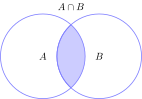
\includegraphics{vennintersection.svg}

The \emph{union} $A\cup B$ is the
set consisting of the elements in $A$ or $B$. To be more precise, an element is in
$A\cup B$ if it is in $A$ or in $B$ (or in both of them):

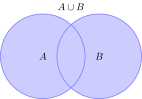
\includegraphics{vennunion.svg}

Lastly, the
difference $A\setminus B$ (between $A$ and $B$) consists of the elements
in $A$ not contained in $B$:

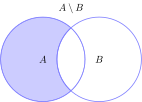
\includegraphics{venndifference.svg}

You should experiment using the Sage window below to get a feeling for these three operations.

\begin{sage}
A = Set([1, 2, 3, 4, 5, 6, 7, 8, 9])
B = Set([7, 8, 9, 10, 11, 12])
print("A =", A)
print("B =", B)
print("The intersection of A and B is ", A.intersection(B))
print("The union of A and B is ", A.union(B))
print("The difference between A and B is ", A.difference(B))
\end{sage}

\beginshex
Let $A = \{1, 2, 3\}$, $B = \{3, 4, 5\}$ and $C = \{0, 1, 5\}$. Verify by hand (no computer) that
\begin{enumerate}[(i)]
\item
  $A\cup B = \{1, 2, 3, 4, 5\}$.
\item
  $A\cap B = \{3\}$.
\item
  $A\cap (B\cap C) = \emptyset$.
\item
  $B\setminus A = \{4, 5\}$.
\item
  $
A \cap (B\cup C) = (A\cap B) \cup (A \cap C).
  $
\end{enumerate}
\endshex

\beginshex
Given two sets $A$ and $B$, is it true that
$A \cap B = B \cap A$ and $A\cup B = B\cup A$?

What about $A\setminus B = B\setminus A$?

Suppose that $A$ and $B$ are two finite sets. Is it true that
$$
|A\setminus B| = |A| - |B|?
$$
What about
$$
|A\cup B| = |A| + |B|?
$$
Seriously, both formulas are wrong. Can you come up with the correct
version of the formula for $|A \cup B|$?

Use your correct formula to find a formula for
$$
|A\cup B \cup C|
$$
viewing $A\cup B$ as the first set and $C$ as the second set. Here you need
the formula
$$
(A\cup B)\cap C = (A\cap C) \cup (B\cap C).
$$
Why is this formula true? Finally, explain why
$$
C \setminus (A\cap B) = (C\setminus A) \cup (C\setminus B).
$$
\begin{hideinbutton}{Hint}
If you are attacking the last part of this exercise using Exercise \ref{logictt}, you
may find it useful to notice that two sets $S_1, S_2$ are equal i.e, $S_1 = S_2$
if and only if
$$
x\in S_1 \iff x\in S_2.
$$
Also,
\begin{align*}
x &\in S_1 \cup S_2 \iff x\in S_1 \lor x\in S_2\\
x &\in S_1 \cap S_2 \iff x\in S_1 \land x\in S_2\\
x &\in S_1 \setminus S_2 \iff x\in S_1 \land x\not\in S_2\\
x &\not\in S_1 \iff \neg (x\in S_1).
\end{align*}
\end{hideinbutton}
\endshex

\beginshex
There is one more operation called the symmetric difference between two sets $A$ and $B$. It is
denoted $A\, \Delta\, B$. Experiment in the Sage window below to find out exactly what it does.
Is it true that $A\, \Delta\, B = B\, \Delta\, A$?

\begin{sage}
A = Set([1,2,3,4])
B = Set([4,5,6,7])
print("A =", A)
print("B =", B)
print("The symmetric difference between A and B is ", A.symmetric_difference(B))
\end{sage}
\endshex

The following is an excerpt from the infamous \emph{Beredskabsprøve Datalogi}.

\begin{quizexercise}[showhide]
\begin{quiz}
\question
Let $X$ and $Y$ denote sets. Which of the following are true?
\answer{T}
$X \cup X = X$
\answer{T}
$X\cap X = X$
\answer{F}
$X\setminus X = X$
\answer{T}
$X\subseteq X\cap X$
\answer{T}
$\emptyset \subseteq X$
\answer{T}
For some sets $X$ and $Y$ we can have
$$
X\cap Y = X\cup Y.
$$
\end{quiz}
\end{quizexercise}



\subsection{Pairs, triples and tuples}

Given two sets $A$ and $B$ we can form the new set $A\times B$,
which is the set of pairs $(a, b)$, where $a\in A$ and
$b\in B$. For example,
$$
\{1, 2\}\times \{1, 2, 3\} = 
\{(1, 1), (1, 2), (1, 3), (2, 1), (2, 2), (2, 3)\}.
$$
The set $A\times B$ is also called the \url{Cartesian
  product}{https://en.wikipedia.org/wiki/Cartesian_product} of $A$ and
$B$.


\beginshex
Consider two pairs $(a, b)$ and $(c, d)$. What is a natural way of defining
equality between these pairs i.e., $(a, b) = (c, d)$?
\endshex

The Cartesian product can be computed in Sage as shown below.

\begin{sage}
A = Set([1, 2])
B = Set([1, 2, 3])
C = cartesian_product([A, B])
print("A =", A)
print("B =", B)
print("The cartesian product of A and B is ", list(C))
\end{sage}

There is no need to restrict ourselves to pairs. We might as well
consider triples $A\times B\times C$ i.e., 
the set of all $(a, b, c)$, where $A$, $B$ and $C$ are sets, or
for that matter general tuples
$$
(a_1, a_2, \dots, a_n)\in A_1\times A_2\times \cdots \times A_n
$$
of any length $n\in \NN$, where $a_1\in A_1, a_2\in A_2, 
\dots, a_n\in A_n$. Based on the above example with tuples we have,
\begin{align*}
&\{0\}\times\{1, 2\}\times \{1, 2, 3\} = \\
&\{(0, 1, 1), (0, 1, 2), (0, 1, 3), (0, 2, 1), (0, 2, 2), (0, 2, 3)\}.
\end{align*}

You may check this using the Sage snippet below.

\begin{sage}
A = Set([0])
B = Set([1, 2])
C = Set([1, 2, 3])
print("A =", A)
print("B =", B)
print("C =", C)
D = cartesian_product([A, B, C])
print("The cartesian product of A, B and C is ", set(D))
\end{sage}

\begin{definition}
For a given set $A$ and $n\in \NN$ we define the $n$-fold cartesian product of $A$ as
$$
A^n = \underbrace{A\times A\times \cdots \times A}_{n\text{ times}}.
$$
\end{definition}

\begin{sage}
A = Set([1,2])
n = 3
B = cartesian_product([A]*n)
print("A =", A)
print("n =", n)
print("The n-fold cartesian product of A is ", set(B))
\end{sage}

\beginshex
Is there an insightful geometric way of drawing the set of pairs given by $\RR^2$? In the same way, is there a geometric
way of thinking of $\RR^3$?
\endshex

\beginshex\label{exprodsets}
Let $A$ and $B$ be two sets. Is $A\times B = B \times A$?

Let $X$ be any set. What is $\emptyset \times X$?

Let $A, B, C$ and $D$ be four sets. Is
$$
(A\times B)\setminus (C\times D) = (A\setminus C)\times (B\setminus D)?
$$

\begin{hint}[showhide]
  See Exercise \ref{sageexsets}.
\end{hint}
\endshex


\beginshex\label{sageexsets}
Use Sage to solve Exercise \ref{exprodsets} by using the code below.

\begin{sage}
A = Set([1,2])
B = Set([2,3])
C = Set([3,4])
D = Set([4,5])
emptyset = Set([])
print(set(cartesian_product([emptyset, B])))
#print(set(cartesian_product([A, B])))
#print(set(cartesian_product([B, A])))
print(set(cartesian_product([A, B])).difference(set(cartesian_product([C, D]))))
print(set(cartesian_product([A.difference(C), B.difference(D)])))
\end{sage}

\endshex

\beginshex
We have silently used \texttt{set} instead of \texttt{Set} in specific places in the Sage windows above.
What is the difference between these two?
\endshex

\section{Ordering numbers}

Let us be a little rigorous and introduce the (usual) ordering
on our numbers with addition and multiplication using almost full blown
mathematical formalities. First the formal definition for two
integers $x, y\in \ZZ$:

\begin{equation}[emph]\label{ordZ}
x \leq y\qquad \text{ means that }\qquad y - x\in \NN
\end{equation}


Notice that $x = y$ implies that $x\leq y$ (and $y\leq x$).
Along this line we also define $x < y$ if $x \leq y$ and $x\neq y$.

\begin{quizexercise}[showhide]
\begin{orderquiz}
  \question
  Assume that $x, y, z\in \ZZ$ and that $x \leq y$. Then drag and drop the
  elements from the left to the right below to explain that
  $x + z \leq y + z$.
  \answer %1
  By assumption $x\leq y$.
  \answer %2
  This means that $z - x + y\in \NN$
  \answer %3
  This means that $y - x\in \NN$
  \answer %4
  To show that $x + z \leq y + z$, we need to show that
  $(y + z) - (x + z) \in \NN$.
  \answer %5
  But $(y + z) - (x + z) = y + z - x + z$. Therefore,
  \answer %6
  But $(y + z) - (x + z) = y + z - x - z = y - x$. Therefore,
  \answer %7
  $(y + z) - (x + z)\in \NN$, since
  \answer %8
  $y - x \in \NN$
  \expected{6}

  \case{(is 134678)}{T}
  \green{Spot on, my friend.}

  \case{(is 467813)}{T}
  \green{This is right!}
  
  \case{(is 413678)}{T}
  \green{This is right!}

  \default
  \red{Wrong order. Check the definition of $\leq$ in \eqref{ordZ} once more!}
\end{orderquiz}
\end{quizexercise}

\beginshex
Suppose \footnote{that}{As an example, this could be assuming $1 \leq 2$ and $2 \leq 5$ and then
    arguing that $1\leq 5$.}
  $$x \leq y\qquad\text{and}\qquad y\leq z
  $$
  for three integers $x, y, z\in \ZZ$. Argue
  from the definition in \eqref{ordZ} that $x\leq z$ by using the definitions of
  $x\leq y$ and $y\leq z$ to conclude that $x\leq z$.
  
  \begin{hint}[showhide]
    The definition of $x\leq z$ is $z-x\in \NN$. The definition of $x\leq y$ is
    $y - x\in \NN$. The definition of $y\leq z$ is $z-y\in \NN$. How do you get from
    the assumptions
    $$
    y - x\in \NN\qquad\text{and}\qquad z - y\in \NN
    $$
    to the conclusion
    $$
    z - x\in \NN?
    $$
    \begin{hint}[showhide]
      If $a\in \NN$ and $b\in \NN$, then $a + b\in \NN$.
    \end{hint}
  \end{hint}
\endshex

\beginshex\label{multposordZ}
Suppose that $x\leq y$ and $a\in \NN$, where $x, y\in \ZZ$. Conclude that 
$$
a x \leq a y.
$$
What if we only assume that $a\in \ZZ$? You are welcome to experiment with
some concrete numbers like $x = 1, y = 2$ and $a = -3$. In the end
you should be able to come up with an argument using the variables
$x, y, a$ with the given assumptions.

\begin{hint}[showhide]
  $a x \leq a y$ means that $a y - a x \in \NN$, but
  $$
  a y - a x = a ( y -  x)
  $$
  and $x \leq y$ means that $y - x\in \NN$.
  
  \begin{hint}[showhide]
    If $a\in \NN$ and $b\in \NN$, then $a b\in \NN$.
  \end{hint}
\end{hint}
\endshex

  


You can
see that this definition agrees with our preconception that
\begin{equation}\label{ordwrong}
\cdots < -3 < -2 < -1 < 0 < 1 < 2 < \cdots
\end{equation}

To be precise, writing $\cdots < -3 < -2 < -1 < 0 < 1 < 2 < \cdots$ is nonsense, since $\leq$ is only defined for two integers in \eqref{ordZ}. 


\begin{exercise}[emph]
  How is one supposed to interpret $0 < 1 < 2$ for example? Go ahead and formulate \eqref{ordwrong} correctly comparing only two integers at a time.
  How does Python/Sage interpret $-3 < -2 < -1< 0 < 1 < 2$? Find out using the Sage snippet below.
  
\begin{sage}
-3 < -2 < -1 < 0 < 1 < 2
\end{sage}
  
  What about $1 < 5 > 3 < 4$? What about $0 < 1 > 2$?
\end{exercise}

Notice that the set of integers has huge holes. Given two integers $a, b\in \ZZ$, such
that $a < b$, we cannot always find an integer $c\in \ZZ$ in between $a$ and $b$:
$$
a < c < b.
$$

The set of rational numbers has the property that they do not have holes. We can
always find an in between number such as $c$ above. But we need a precise way
of comparing rational numbers. A way to explain precisely why for example
$$
\frac{2}{3}\,\, \leq \,\, \frac{5}{7}.
$$
Of course, you can enter the two numbers a on computer and see that
$\frac{2}{3}$ is approximately $0.67$ and $\frac{5}{7}$
is approximately $0.71$, but we aim for the mathematical
precise definition.

A
rational number $\frac{a}{b}$ is represented by a numerator $a\in \ZZ$ and a denominator
$b\in \ZZ$ with $b > 0$. We already know the criterion for two rational numbers
$\frac{a}{b}$ and $\frac{c}{d}$
to be \footnote{equal}{Technically speaking we are defining a socalled \emph{equivalence relation} identifying the infinitely many ways of writing a rational number into one.}:

\begin{equation*}[emph]
\frac{a}{b}\, =\, \frac{c}{d}\qquad \text{ means that }\qquad a d = b c\qquad (\text{in }\ZZ).
\end{equation*}


We wish to compare the two rational numbers $\frac{a}{b}$ and $\frac{c}{d}$ deciding
precisely how they are ordered:

\begin{equation}[emph]\label{defcompQQ}
\frac{a}{b}\, \leq\, \frac{c}{d}\qquad \text{ means that }\qquad a d \leq b c\qquad (\text{in }\ZZ).
\end{equation}


\begin{frameit}
\begin{remark}
  How does one come up with the definition in \eqref{defcompQQ}? Why not
  $a^3 b^2 + b^7 \leq a b^8 - a$ instead of $a d \leq b c$? The reason is that
  we want the order on $\QQ$ to be related to the one we already defined on
  the subset $\ZZ\subseteq \QQ$. It should respect multiplication by positive numbers just
  as in Exercise \ref{multposordZ}. If we want this to hold, we are forced
  to the definition in \eqref{defcompQQ}, since
  $$
  (b d)\,\frac{a}{b} = a d\qquad\text{and}\qquad (b d)\, \frac{c}{d} = b c.
  $$
\end{remark}
\end{frameit}


  


As for the integers, we also define $x < y$ if $x \leq y$ and $x\neq y$ for
two rational numbers $x$ and $y$.

Using this definition, you can check that $\frac{2}{3} \leq \frac{5}{7}$, since
$$
2\cdot 7 < 3 \cdot 5.
$$
 
An easy, but surprising, 
way of finding a rational number strictly between these two is
adding their numerators and denominators:
$$
\frac{2}{3} < \frac{2 + 5}{3 + 7} < \frac{5}{7}.
$$

We wil try to explain the first inequality in mathematical general terms going through a
rather formal proof consisting of five steps. These steps are
given in the quiz below. Your task is to drag from the left and drop them to the right in an order, 
so that the proof makes sense. 

After that you are supposed, on your own, to write down a precise proof of
the second inequality.

\begin{quizexercise}[showhide]
\begin{orderquiz}
  \question
  Order the arguments below so that they constitute a coherent explanation of the
  statement that if
  $$
  \frac{a}{b} < \frac{c}{d},
  $$
  then
  $$
  \frac{a}{b} < \frac{a + c}{b + d}
  $$

  
  \answer %2
  By definition this means that $a d < b c$.

  
  
 \answer %1
  We are assuming that $\frac{a}{b} < \frac{c}{d}$. 

  \answer %4
  For integers $x, y, z$ we know that the rule
  $
  x ( y + z) = x y + x z
  $
  holds. Therefore
  \answer %5
  we need to show that $a b + c d < b a + b c$.

  
  \answer %6
  Since $a b = b a$ and $a b + a d < a b + b c$ is a consequence of $a d < b c$, we are
  done if we know this is true.
  \answer %7
  However, this is a consequence of our assumption $\frac{a}{b} < \frac{c}{d}$.

\answer %3
  To show that
  $
  \frac{a}{b} < \frac{a+c}{b + d},
  $
  we need to argue that $a (b + d) < b (a + c)$.

  
  \answer

  we need to show that $a b + a d < b a + b c$.
  
  \expected{5}

  \case{(is 73856)}{T}
  \green{Spot on, my friend!}

  \case{(contains 4)}{F}
  \red{You have not applied the formula for expanding $x(y + z)$ correctly.}

  \default
  \red{Wrong order.}

\end{orderquiz}
\end{quizexercise}




\beginshex
Similarly to the quiz above, assume that  
$$
  \frac{a}{b} < \frac{c}{d}.
  $$
  Write down a precise argument showing that
  $$
  \frac{a + c}{b + d} < \frac{c}{d}.
  $$
  You may seek inspiration in Video \ref{Video:proofexample} for
  how to mix math and words (even though
  it is further ahead).
  \endshex

  
  

\beginshex
On \url{Twitter}{https://twitter.com/Ramangupta4/status/1162999733142482945}, Raman Gupta posted the note below

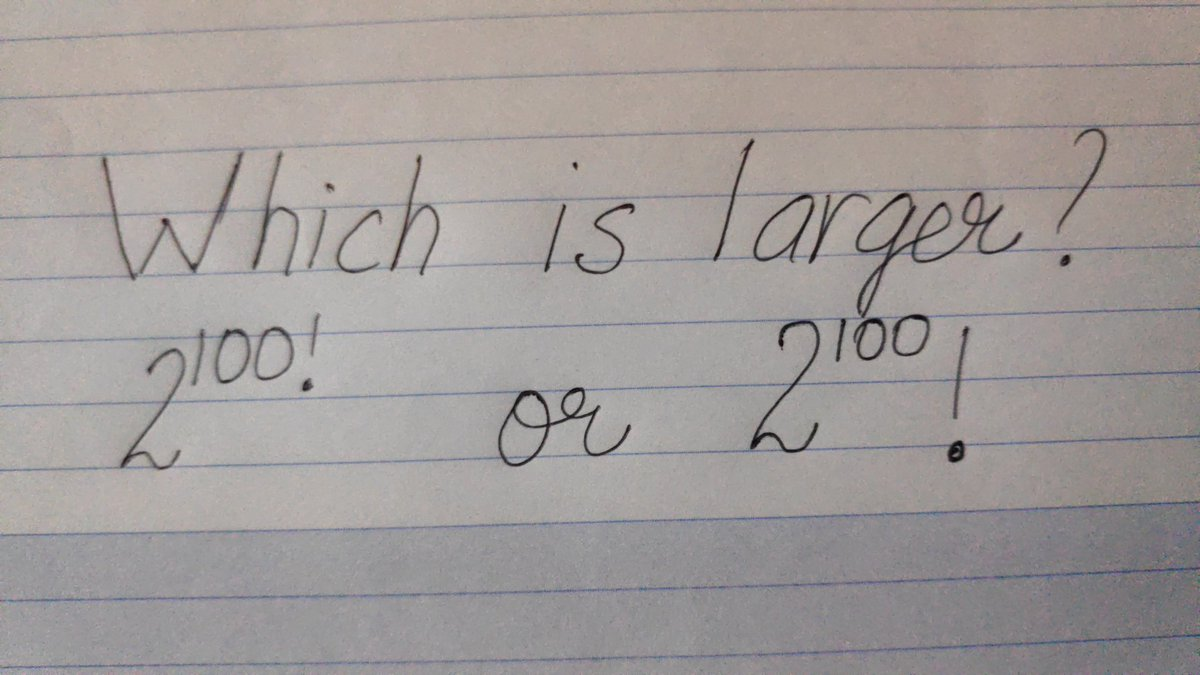
\includegraphics[width="50\%"]{tweet.jpg}

For a natural number $m\in \NN$,
$$
m! = m (m-1) (m-2)\cdot \dots \cdot 2\cdot 1. 
$$
For example, $3! = 6$ and $5! = 120$. What is the answer for the
question in the note?

\begin{hint}[showhide]

Experiment a bit with Sage: define a function $f(n)$, which computes
$$
2^{n!} - 2^n!
$$

Then look at

$$
f(1), f(2), f(3), f(4), f(5), \dots
$$

\end{hint}
\endshex

The exercise below shows that our trick for finding rational numbers
in between two given rational numbers can be made into a machine for
generating all positive rational numbers!

\beginshex
Can you spot the system in the fractions in the diagram below?
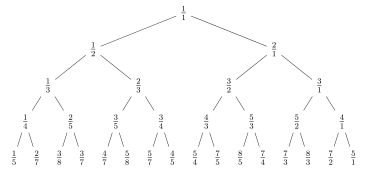
\includegraphics{SternBrocotTree.svg}
Once you see the system, extend the diagram with the next level downwards. Is every
positive fraction present in this diagram if one keeps adding levels?

\begin{hint}[showhide]
Suppose that
$$
\frac{p}{q} < \frac{r}{s}
$$
and $q r - s p = 1$. Then for
$$
\frac{p}{q} <  \frac{p+r}{q+s} < \frac{r}{s},
$$
we have $q (p+r) - (q+s) p = 1$ and $(q+s) r - (p + r) s = 1$. If $\frac{a}{b}$ is 
a positive fraction, such that
$$
\frac{p}{q} <  \frac{a}{b} < \frac{r}{s},
$$
show that 
$$
a + b = (r+s)(q a - b p)+(p+q)(b r - a s)\geq p+q+r+s.
$$
\end{hint}
\endshex


\subsection{Subsets of numbers and first elements}\label{subsecfirst}

In a set equipped with an order, it is intuitively clear what a first element should be. For example,
the natural numbers $\NN$ has $0$ as its first element. On the other hand the set $\ZZ$ of
integers does not have a first element (it is "infinite to the left").

In fact every non-empty subset $S\subseteq \NN$ has
a first element. This follows from a rather special property of $\NN$: there
can be only finitely many natural numbers smaller than a given one. This is
not true for $\ZZ$. Here there are infinitely many integers smaller than
any integer.

\begin{frameit}[emph]
If $A$ is a set with an order $\leq$ and $B\subseteq A$ is a subset, then formally $x\in B$ is a
first element of $B$ if $x \leq y$ for every element $y\in B$.
\end{frameit}

  



\beginshex
Give an example of a subset of $\ZZ$ that does not have a first element. Does the
subset of even numbers have a first element? Does the empty subset have a first element?
\endshex

\beginshex
Can a non-empty subset of a set with an order have two different first elements? I need to
be precise here. I am assuming that the order $\leq$ (naturally) satisfies: if
$x$ and $y$ are two elements from the subset and $x\leq y$ and $y \leq x$ both hold,
then $x = y$.

Do the orders we defined on $\ZZ$ and $\QQ$ satisfy the above property?

\begin{hint}[showhide]
  If $x \leq y$, where $x, y\in \ZZ$, then $y - x\in \NN$. If $y \leq x$, then $x - y\in \NN$.
  But
  $$
  y - x = - (x - y).
  $$
  In other words, $z = y - x$ is an integer that satisfies $z\in \NN$ and $-z\in \NN$.
  What integer is $z$?
\end{hint}
\endshex

\beginshex
Consider the subset $S$ of $\QQ$ consisting of positive fractions i.e., rational numbers  $>0$.
Does this subset have a first element?
\endshex




\section{Propositional logic}

We have seen quite a few mathematical statements that ended up 
being true or false. Such statements are called \emph{propositions}.
Here are two examples of propositions usings sets (in Sage):

\begin{sage}
print(1 in Set([1,2,3]))
A = Set([1, 2, 3])
B = Set([2, 3, 4])
print(A.intersection(B) == Set([2, 3])) 
\end{sage}

\beginshex
What exactly are the two propositions in the above Sage window written
up in mathematical terminology? Notice that the symbol == is
a programming construct. It is not used in mathematics notation.
\endshex

Propositions can be combined into
new (compound) propositions. Take for example the propositions

\begin{align*}
&p: \text{it rains}\\
&q: \text{it is cloudy}.
\end{align*}
  
  Then ($p$ and $q$) is a perfectly good
  new proposition reading \emph{it rains and it is cloudy}. The same goes for (if $p$ then $q$), which reads
  \emph{if it rains then it is cloudy}. The proposition (if $q$ then $p$) reads \emph{if it is cloudy then
    it rains}. This proposition is (clearly) false.



We need some notation to describe these compound propositions:

\begin{equation*}
\begin{array}{ll}
p \land q\qquad\qquad & \qquad\qquad p \text{ and } q\\
\\
p \lor q\qquad\qquad & \qquad\qquad p \text{ or } q\\
\\
p\implies q\qquad\qquad & \qquad\qquad \text{if } p \text{ then } q\\
\\
\neg p\qquad\qquad & \qquad\qquad \text{not } p
\end{array}
\end{equation*}

The compound propositions are either true($t$) or false ($f$) depending on
$p$ and $q$. The dependencies are displayed in the \emph{truth tables} below.

\begin{equation*}[emph]
\def\arraystretch{1.2}
      \begin{array}{c|c|c}
        p & q  & p\land q  \\
        \hline 
        t & t  & t    \\
        t & f & f\\
        f & t & f\\
        f & f & f
      \end{array}\qquad
      \begin{array}{c|c|c}
        p & q  & p\lor q  \\
        \hline
        t & t  & t    \\
        t & f & t\\
        f & t & t\\
        f & f & f
      \end{array}
      \qquad
      \begin{array}{c|c|c}
        p & q  & p\implies q  \\
        \hline
        t & t  & t    \\
        t & f & f\\
        f & t & t\\
        f & f & t
      \end{array}\qquad
      \begin{array}{c|c}
        p & \neg p \\
        \hline
        t & f\\
        f & t
      \end{array}
  \end{equation*}


The tables for the compound propositions $p\land q, p\lor q$ and also
$\neg p$ are not too hard to grasp. The table for $p\implies q$ 
raises a few more questions. Why is $f\implies t$ true?
I will not go into this, but just point out that there are
many explanations available online and, 
perhaps more importantly, refer you to Exercise \ref{excolorcards} and the remark below.



\begin{frameit}
  \begin{remark}
    Here is a statement about real numbers
    \begin{equation}\label{exampleimplies}
    x > 0 \qquad \implies \qquad x^2 > 0.
    \end{equation}
    This statement reads: no matter which real number $x$ you pick, if $x > 0$,
    then $x^2 > 0$. We definitely want this to be true. Being true means
    that \eqref{exampleimplies} must hold for all numbers $x$, also $x = -7$,
    which reads
    $$
    - 7 > 0 \qquad \implies \qquad (-7)^2 = 49 > 0.
    $$
    The above statement is an example of a false implies true statement, which
    we want to be true: even though $-7$ is negative, its square is positive.

    In general terms, in proving the statement that $p(x) \implies q(x)$ holds for every $x$ in
    some set $S$, we are really only interested in $x\in S$ for which $p(x)$ is true, since
    $p(x)$ is our assumption. We still need $p(x)\implies q(x)$ to be true for $x\in S$ for
    which $p(x)$ is false. This is assured by the truth table for $\implies$, since 
    $f \implies t$ and $f\implies f$ are both true.
  \end{remark}
\end{frameit}


We may also check what Sage outputs for the truth table of $p\implies q$ (or for that
matter \footnote{any formula}{Notice that Sage uses \texttt{->} for $\implies$, \texttt{\&} for $\land$, \texttt{|} for $\lor$ and \texttt{~} for $\neg$.}.
 combining the logical operations above):

\begin{sage}
f = propcalc.formula("p->q")
print(f.truthtable())
g = propcalc.formula("~q->~p")
print(g.truthtable())
h = propcalc.formula("~(p|q)")
print(h.truthtable())
i = propcalc.formula("~p & ~q")
print(i.truthtable())
\end{sage}

  



\beginshex\label{excolorcards}
Suppose that we are presented with four cards
\begin{equation}\label{cards}
\boxed{3}\qquad \fcolorbox{black}{red}{\phantom{3}}
\qquad\boxed{4}\qquad \fcolorbox{black}{blue}{\phantom{4}}
\end{equation}
with a (natural) number on the front and the color
\textcolor{blue}{blue} or \textcolor{red}{red} on the back.
In \eqref{cards}, the first and third cards are shown with their fronts facing up and
the second and fourth cards are shown with their backs facing up.

A claim (proposition) is made that if a card has an even number on the front, then it
must have the color \textcolor{blue}{blue} on the back.

Your task is to verify this for the cards above. Of course you can
do this by turning all four cards, but is there a way of checking this
by turning less than four cards?

What if we add the claim, that if a card has the color 
\textcolor{blue}{blue} on the back, then
it must have an even number on the front?

\begin{hint}[showhide]
  Find two propositions $p$ and $q$ so that the claim reads
  $p\implies q$.
\end{hint}
  
\endshex


\beginshex
Explain why Python/Sage thinks that \footnote{the value}{Thanks to Gerth Brodal for pointing this out to me} of
  $$
  1 < 0 < 1/0
  $$
  is False! Notice that you are dividing one by zero in the last "integer" above.
\endshex


In the exercise below you will see for example that
$p\implies q$ is the same as $\neg q \implies \neg p$.

\beginshex\label{trutheq}
Two propositions are considered the same ($=$) if they have the same truth table. Verify, by
filling out and comparing truth tables, that
\begin{enumerate}[(i)]
\item
$\neg (p \land q) = (\neg p) \lor (\neg q)$
\item
$\neg (p \lor q) = (\neg p) \land (\neg q)$
\item
$p \implies q = (\neg q) \implies (\neg p)$
\item
$p \implies q = (\neg p)\lor q$
\end{enumerate}
\endshex

\beginshex\label{logictt}
Can you use the setup up in Exercise \ref{trutheq} to verify that
$$
p\land (q \lor r) = (p\land q) \lor (p \land r)
$$
for three propositions $p, q$ and $r$? What about
$
p\lor (q \land r)?
$
\endshex

The notation $p \iff q$ is used frequently. It means that both
$p\implies q$ and $q\implies p$ are true i.e.,
$$
(p\implies q) \land (q\implies p).
$$





\subsection{The symbols $\exists, \forall$ and propositions with variables}

In mathematics one usually reasons with propositions with variables.

In order to have a variable $x$, one must first specify to which set
$S$ the variable belongs. For example, the proposition $p(x)$ given by
$$
x^2 > 0,
$$
does not make sense if $x$ is taken from the set of letters in the
English alphabet (not unless you give an interpretation of $x^2$,
$>$ and $0$ in this set). However, if $x\in \ZZ$, then $p(x)$
certainly makes sense. Whether $p(x)$ is true depends on $x$.


For example, $p(0)$ is false, whereas $p(-1)$ is true. This leads us to
the existential and universal quantifiers $\exists$ and $\forall$.
The former reads \emph{there exists} and the latter \emph{for every}.

For example, the proposition
$$
\exists x\in \ZZ: \neg p(x)
$$
is true and so is
$$
\forall x\in \ZZ\setminus\{0\}: p(x).
$$
Notice that the  symbol ":" above means \footnote{"such that"}{Therefore  
$\exists x\in \ZZ: \neg p(x)$ reads "there exists $x$ in $\ZZ$, such that
$\neg p(x)$ is true".}.

Also, $\forall x\in \ZZ: p(x)$ is false, because
$\exists x\in \ZZ: \neg p(x)$ is true. In general,
$$
\neg\left(\forall x\in S: p(x)\right) = \exists x\in S: \neg p(x).
$$
So we do not really need the quantifier $\forall$, when we have
$\neg$ and $\exists$, but $\forall$ is convenient and used all
the time.

The quantifiers are important to learn and apply when expressing
mathematical ideas. So is the use of propositions with variables
in writing up subsets: if $S$ is a set, $x$ a variable taking values
in $S$ and $p(x)$ a proposition (making sense in $S$), then
$$
\{x\in S \mid p(x)\}
$$
is the subset of the elements $x\in S$, such that $p(x)$ is true.

For example, if $p(x) = x^2 > 0$, then
$$
\{x\in \ZZ \mid p(x)\} = \ZZ\setminus \{0\}.
$$

Suppose that $p_1(x), \dots, p_n(x)$ are propositions with a variable $x$ taking values
in $S$, then we often use the notation
$$
\{x\in S \mid p_1(x), \dots, p_n(x)\}
$$
for
$$
\{x\in S \mid p_1(x)\land \dots\land p_n(x)\}.
$$

\begin{remark}[emph]\label{remarkseveralvars}
  It also makes sense to have propositions in more than one variable. With
  variables $x, y$ in $\NN$, such a proposition $q(x, y)$ could be
  $$
  x\text{ and }y\text{ are prime numbers and } x + y \text{ is a prime number}.
  $$
\end{remark}

\beginshex
Consider the proposition $q(x, y)$ from Remark \ref{remarkseveralvars}. Write
down the elements in
$$
\{(x, y)\in \NN\times \NN \mid q(x, y) \land x + y \leq 10\}.
$$
Is
$$
\{(x, y) \in \NN\times \NN\mid q(x, y)\}
$$
an infinite set?
\endshex

\beginshex
List the elements in the following subsets.
\begin{enumerate}[(i)]
  \item
$$
\{x\in \ZZ \mid x^2 < 10\}.
$$
\item
  $$
  \{(x, y)\in \ZZ\times \ZZ \mid x^2 + y^2 < 5\}.
  $$
\end{enumerate}
\endshex

\beginshex
You have previously encountered systems of linear equations like
\begin{align}\label{exlineqs}
  x + y &= 3\\
  3x - y &=  5. 
\end{align}
The solutions to \eqref{exlineqs} can be identified with a subset of
$\RR^2$. Define this subset precisely i.e., write the subset as
$$
\{(x, y)\in \RR^2 \mid p(x, y)\},
$$
where $p(x, y)$ is a proposition in the variables $x, y\in \RR$.
\endshex

\beginshex
Suppose that $X = \RR$ and
$$
Y = \{x\in \RR \mid x > 0,\, x < 2\}.
$$
Then write down precisely what $X\setminus Y$ is i.e., find a proposition $q(x)$
in the variable $x$, such that
$$
X\setminus Y = \{x\in \RR \mid q(x)\}.
$$
\endshex

\beginshex
Consider the subset $S$ of $\RR^2$ pictured in the drawing below

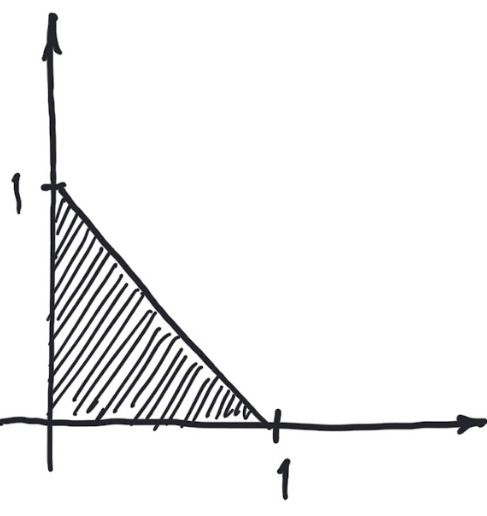
\includegraphics{trianglelogic.png}

Express $S$ as
$$
S = \{(x, y)\in \RR^2 \mid p_1(x, y), p_2(x, y), p_3(x, y)\},
$$
where $p_1, p_2, p_3$ are predicates in the variables $x, y$.

\begin{hideinbutton}{Hint}
  A predicate in the variables $x, y$ could be something like
  $$
  x -y \geq 17.
  $$
\end{hideinbutton}

Express $\RR^2\setminus S$ as
$$
\{(x, y)\in \RR^2 \mid p(x, y)\},
$$
where $p$ is a suitable predicate in the variables $x, y$.
\endshex

The following is yet another excerpt from the infamous \emph{Beredskabsprøve Datalogi}.

\begin{quizexercise}[showhide]
\begin{quiz}
\question
Which of the following are true?
\answer{F}
$\forall x\in \NN: x > 2$
\answer{T}
$\exists x\in \NN: x > 2$
\answer{T}
$\forall x\in \emptyset: x = 7$
\answer{F}
$\exists x\in \emptyset: x = 7$
\end{quiz}
\end{quizexercise}

\subsection{The use of implication ($\implies$) and bi-implication ($\iff$)}

Usually $\implies$ and $\iff$ are applied to link propositions in a logical argument. An example
is
$$
x \leq y \iff x + z \leq y + z
$$
for integers $x, y, z$. To be completely precise, I should here write
$$
\forall x, y, z\in \ZZ: x \leq y \iff x + z \leq y + z,
$$
but one often writes $\forall$ with words as for example \emph{for integers $x, y, z$}.


Here $x \leq y\implies x + z \leq y + z$ is true and similarly
$x + z \leq y + z \implies x \leq y$ (by using the definition (see \eqref{ordZ}) of $\leq$ in $\ZZ$). So the
use of $\iff$ is valid.

However, for $x \geq 0 \implies x^2 \geq 0$ we cannot link the two propositions by $\iff$,
simply because $x^2 \geq 0 \implies x \geq 0$ is false (for $x= -1$).


\section{What is a mathematical proof?}


Most professional mathematicians rarely think about the precise
definition of a proof. During many years of training they have
assimilated knowledge by experience. Therefore many proofs
seem born out of witchcraft containing several magical
devices.

However, many proofs appearing in
respected mathematical journals, submitted by respected mathematicians, have turned out to contain
errors. Recent developments in automated proof systems
like \url{Coq}{https://en.wikipedia.org/wiki/Coq} and \url{LEAN}{https://en.wikipedia.org/wiki/Lean_(proof_assistant)} show
promise in checking proofs like for example the famous
\url{four color theorem}{https://en.wikipedia.org/wiki/Four_color_theorem}.

Informally a proof of a proposition $q$, consists in arguing that an implication $p\implies q$ is true by first assuming $p$. Usually this is done
not only through one implication $p\implies q$, but through a series
of intermediate implications
$$
p\implies q_1 \implies q_2 \implies q_3 \implies \cdots \implies q_N,
$$
where the last proposition $q_N$ is $q$. If $p$ is true, this
will constitute a proof that $q_N = q$ is true. Just like in \eqref{ordwrong},
there is an imprecision here. Can you tell what it is?

In this section we will illustrate a simple mathematical proof of the
proposition:
$$
\forall n\in \NN: p(n)\implies p(n^2),
$$
where $p(n) = (n\text{ is odd})$ i.e., the square of an odd
natural number has to be odd. This seems true for a first selection
of examples: $3^2=9, 5^2=25, \dots$.

First we need to know what $p(n)$ means. What does it mean
exactly for a number to be odd? This means that it is
not divisible by $2$ or that there exists another
natural number $a$, such that $n = 2 a + 1$. So
$$
p(n) = \exists a\in \NN: n = 2 a + 1.
$$
Therefore we need to show that
$$
\left(\exists a\in \NN: n = 2 a + 1\right) \implies
\left(\exists b\in \NN: n^2 = 2 b + 1\right).
$$
Notice that I had to change $a$ into $b$ in the second proposition above.
The two variables are not the same: $a$ is associated with $n$ and
$b$ is associated with $n^2$.

Let us assume that $n = 2 a + 1$. Now we need to argue that $
n^2 = 2 b + 1$ for some $b\in \NN$. You stare at this for a while
and notice that we should use the assumption $n=2 a + 1$ in
computing $n^2$:
$$
n^2 = (2 a + 1)^2 = (2 a)^2 + 2 (2 a) + 1^2 = 4 a^2 + 4 a + 1 =
2(2 a^2 + 2 a) + 1.
$$
Thus, using our assumption we may conclude that if $n = 2 a + 1$, then
$$
n^2 = 2 b + 1,
$$
where $b=2a^2+ 2 a$. This completes the proof.

The beauty here is that we have verified for all odd natural numbers
that their square is odd. Not just a finite selection like
$3, 7, 11, 13$.

Below I have given a very detailed walk through of the proof above. It
examplifies how to write up the proof mixing words and mathematics. In
many ways a proof is like a detailed argument in a court case, except
that the rules of mathematics are universal. You need the absolute truth.

\begin{video}\label{Video:proofexample}
\youtube{1tewESCAP2k}  
\end{video}




\subsection{Proof by contradiction}

A proposition $p$ is either true or false. This seemingly obvious statement
goes by the name of \emph{the law of excluded middle} and dates back to the writings
of \url{Aristotle}{https://en.wikipedia.org/wiki/Aristotle}.


\begin{example}
  An irrational number is a (real) number that is not rational. It is a
  startling fact that such numbers exist, but they do! The \url{square root $\sqrt{2}$ of two}{https://en.wikipedia.org/wiki/Square_root_of_2}
  is an example. 
  We will prove that there exists two irrational numbers $\alpha, \beta$, such that
$\alpha^\beta$ is rational.

  Consider the proposition $p$ given
  by
  $$
  \gamma = \sqrt{2}^{\sqrt{2}}\text{is rational.} % \text{\ is rational} gives AttributeError: 'TokenType' object has no attribute 'rege'
  $$
  Either $p$ is true or false. If $p$ is true we are done putting $\alpha = \beta = \sqrt{2}$. If not, then
  $p$ must be false and $\gamma$ is irrational. But then
  $$
  \gamma^{\sqrt{2}} = \left(\sqrt{2}^{\sqrt{2}}\right)^{\sqrt{2}} = (\sqrt{2})^{\sqrt{2}\cdot \sqrt{2}} = \sqrt{2}^2 = 2
  $$
  and we are done putting $\alpha = \gamma$ and $\beta = \sqrt{2}$.
\end{example}

\beginshex
We know that $\sqrt{2}^2$ is $\sqrt{2}$ multiplied by itself, but can you define $\sqrt{2}^{\sqrt{2}}$ in a similar
precise way?

\begin{hint}[showhide]
  Here you need help from the special functions $e^x$ and $\log(x)$.
\end{hint}
\endshex

\beginshex
So which one is it? Is
$$
\sqrt{2}^{\sqrt{2}}
$$
rational or irrational? 

\begin{hint}[showhide]
  This is advanced mathematics! Try to make sense of the famous
  \url{Gelfond-Schneider theorem}{https://en.wikipedia.org/wiki/Gelfond\%E2\%80\%93Schneider_theorem}.
  \end{hint}
\endshex

The law of excluded middle can be turned
into a powerful proof technique called \emph{proof by contradiction}.

Suppose we wish to establish that $p$ is true. Then we turn things upside down by
assuming that $p$ is false i.e., that $\neg p$ is true. If we then
by logical deduction can show that
$$
\neg p \implies q,
$$
for some proposition $q$, which is demonstrably false, then $\neg p$ cannot be true (since
true $\implies$ false is false). Therefore $\neg p$
must be false and $p$ must be true by the law of the excluded middle. This technique is used all the time!

Perhaps the two most famous proofs by contradiction in all of mathematics are due to \url{Euclid}{https://en.wikipedia.org/wiki/Euclid}. The first one is about the \url{infinitude of the prime
  numbers}{https://en.wikipedia.org/wiki/Euclid\%27s_theorem}.
Here one assumes to begin with that
there are finitely many prime numbers and follows this through to a contradiction.
See Exercise \ref{exprimeinfinite}.




The second
one (perhaps even attributable to Artistotle) is about \url{the irrationality of $\sqrt{2}$}{https://en.wikipedia.org/wiki/Square_root_of_2#Proof_by_infinite_descent}. Here one assumes to begin with
that $\sqrt{2}$ is rational and follows this through reaching a contradiction. See
Exercise \ref{exsqrt2notrat}.


\begin{example}
  We will give an example of a proof by contradiction using a previous exercise: let $p$
  be the proposition that
the subset
$$
S = \{x\in \QQ \mid x > 0\}
$$
of $\QQ$ 
does not have a first element. Recall the definition of a first element in
the context of $S$: $x_0\in S$ is a first element if 
$$
\forall x\in S: x_0 \leq x.
$$
So if $x_0$ is a first element in $S$, there cannot exist $x_1\in S$, such that
$x_1 < x_0$.

The proof by contradiction  in this case, runs as follows. Assume $\neg p$ i.e., that $S$
has a first element say
$$
x_0 = \cfrac{a}{b}.
$$
Then using $x_0$ we can form
$$
x_1 = \frac{a}{b+1},
$$
and you \footnote{can check}{Check that $a b < a(b+1)$.} that $x_1\in S$ and $x_1 < x_0$ i.e., $x_0$ is not a first
element. So our assumption that $S$ has a first element immediately leads
to the conclusion that $S$ does not have a first element. In fact, we have proved
$$
\neg p \implies p.
$$
Therefore $\neg p$ (the wrong assumption)
has to be false and thus $p$ must be true.
\end{example}

\beginshex\label{exprimeinfinite}
Consider the first $n$ prime numbers
$$
p_1 = 2, p_2 = 3, p_3 = 5, \dots, p_n.
$$
Check that
\begin{align*}
  &p_1\\
  &p_1\, p_2 + 1\\
  &p_1\, p_2\, p_3 + 1\\
  &p_1\, p_2\, p_3\, p_4 + 1
\end{align*}
are prime numbers by using the Sage window below (\texttt{factor} gives
the prime factorization of a natural number).

\begin{sage}
  factor(30)
\end{sage}

Is it true in general that
$$
p_1\, p_2\, \cdots \, p_n + 1
$$
is a prime number?

Assume that we know that every natural number must be divisible by a prime number. Show how the
assumption that there are only finitely many prime numbers say
$$
p_1, p_2, \dots, p_n
$$
leads to a contradiction by using that the natural number
$$
p_1\, p_2\, \dots\, p_n + 1
$$
must be divisible by a prime number.
\endshex

\beginshex\label{exsqrt2notrat}
Suppose that $q(n) = (n \text{ is even})$. Prove that
$$
\forall n\in \NN: q(n^2) \implies q(n).
$$
Suppose that
$$
\sqrt{2} = \frac{m}{n}.
$$
Show that this implies $2 n^2 = m^2$ and that $m$ and $n$ are even numbers.

Given the above, write up a precise proof that $\sqrt{2}\not\in \QQ$
using proof by contradiction.

You may wonder what is so special about rational numbers. Which property does
$\sqrt{2}$ break? You can explore this by looking at the decimal expansion of
some fractions below.

\begin{sage}
print("1/8 =", (1/8).n(digits=50))
print("3/17 = ", (3/17).n(digits=50))
print("5/7 = ", (5/7).n(digits=50))
print("")
print("sqrt(2) = ", sqrt(2).n(digits=100))
\end{sage}

However, $\sqrt{2}$ is an algebraic number being a root in the
polynomial $x^2 - 2$. In general an algebraic number is a number,
which is a root in a polynomial with coefficients in $\ZZ$.

\endshex


\subsection{Proof by induction}

A precocious Gauss proved the formula
\begin{equation}\label{gaussind}
1 + 2 + \cdots + n = \frac{n(n+1)}{2}
\end{equation}
at the age of seven displaying remarkable ingenuity for his age. Lesser
mortals usually use induction to prove this formula. Gauss was asked
along with his classmates to compute the sum of all natural numbers
$1, 2, \dots, 100$. Using his formula he quickly came up with the correct
answer $5050$. His classmates had to work for the entire lesson.

Suppose that the formula in \eqref{gaussind} is viewed as a
proposition $p(n)$. To prove the formula we need to prove it for all
natural numbers (you can easily see that $p(1)$ and $p(2)$ are true) i.e.,
we need to prove
$$
\forall n\in \NN\setminus\{0\}: p(n).
$$
An induction proof is a way of proving this statement by showing two things:
\begin{enumerate}[(i)]
\item
  $p(1)$
\item
  $\forall n\in \NN\setminus\{0\}: p(n)\implies p(n+1)$
\end{enumerate}
These two statements ensure that $p(1) \implies p(2)$. Therefore
$p(2)$ must be true, since we assumed $p(1)$ true from the
beginning. Similarly $p(2)\implies p(3)$ ensures that $p(3)$
is true and so on. In fact we have proved $p(n)$ for every $n\in \NN$
using this technique. One can prove this using proof by
contradiction and that every non-empty subset
of $\NN$ has a first element (see subsection \ref{subsecfirst} and below).

\begin{theorem}[emph]\label{thminduction}
  Suppose that $p(n)$ are infinitely many propositions given by $n\in \NN\setminus\{0\}$. Then
  $$
  \forall n\in \NN\setminus\{0\}: p(n)
  $$
  is true if
\begin{enumerate}[(i)]
\item
  $p(1)$ is true.
\item
  $\left(\forall n\in \NN\setminus\{0\}: p(n)\implies p(n+1)\right)$ is true.
\end{enumerate}
\end{theorem}

\begin{proof}[showhide]
Suppose by contradiction that there exists $n\in \NN\setminus\{0\}$, such that
$p(n)$ is false. Then the subset
$$
S = \{n\in \NN \mid \neg p(n)\}\subseteq \NN
$$
is non-empty. Therefore it has a first element $n_0\in S$. 
Here $n_0 > 1$, since $p(1)$ is assumed to be true. So we
know that $p(n_0-1)$ is true and that
$p(n_0-1)\implies p(n_0)$ is true. But the latter
implication is a contradiction, since true implies
false is false.
\end{proof}

\beginshex
What happens if $\NN\setminus\{0\}$ is replaced by $\NN$ and $p(1)$ by $p(0)$ in Theorem \ref{thminduction}?
\endshex


Let us see how an induction proof plays out in the above example
with the statement $p(n)$ that
\begin{equation}\label{indant}
1 + 2 + \cdots + n = \frac{n(n+1)}{2}.
\end{equation}
Clearly $p(1)$ is true. We need to prove $p(n)\implies p(n+1)$, so
we assume that $p(n)$ holds i.e., that \eqref{indant} is true.
Then we may add $n+1$ to both sides of \eqref{indant} to get
$$
1 + 2 + \cdots + n + (n+1) = \frac{n(n+1)}{2} + (n+1).
$$
Here the right hand side can be rewritten as
$$
\frac{n(n+1) + 2(n+1)}{2} = \frac{(n+1)(n+2)}{2},
$$
which is exactly what we want. This is the conjectured formula for
the sum of the numbers $1, 2, \dots, n, n+1$. Therefore
we have proved that $p(n)\implies p(n+1)$ and the induction
proof is complete.



\begin{example}\label{examplegeomseries}
  For a real number $r\neq 1$, the extremely useful formula
  \begin{equation}\label{geoind}
  1 + r + \cdots + r^n = \frac{1 - r^{n+1}}{1-r}
  \end{equation}
  holds. Let us prove this formula by induction. For $n=1$ this amounts to the identity
  $$
  1 + r = \frac{1-r^2}{1-r},
  $$
  which is true since $1-r^2 = (1+r)(1-r)$. We let $p(n)$ denote
  the identity in \eqref{geoind}. We have seen that $p(1)$ is true. The induction step
  consists in proving $p(n)\implies p(n+1)$. We can prove this
  by adding $r^{n+1}$ to the right hand side in \eqref{geoind}:
  \begin{equation}\label{qseriesindstep}
  \frac{1 - r^{n+1}}{1-r} + r^{n+1} = \frac{1 - r^{n+1} + (1-r) r^{n+1}}{1-r} = \frac{1 - r^{n+2}}{1-r}.
  \end{equation}
\begin{hideinbutton}{Real life application}
    In order to pay for a house you borrow $P$ DKK at an interest of
    $r$ per year. You want to pay off your debt over $N$ years by
    paying a fixed amount each year. How much is the fixed yearly
    amount you need to pay?

    Let us analyze the setup: suppose that the fixed yearly amount
    is $Y$. We will find an equation giving us $Y$ in terms of
    $P, N$ and $r$. Put $q = 1+ r$.

    After one year you owe
    $$
    q P - Y.
    $$
    After two years you owe
    $$
    q(q P - Y) - Y.
    $$
    After three years you owe
    $$
    q ( q ( q P - Y) - Y) - Y.
    $$
    In general after $n$ years you owe
    $$
    q^n P - Y (1 + q + \cdots + q^{n-1}).
    $$
    Since we want to be debt free after $N$ years, the yearly payment will have to satisfy
    $$
    q^N P = Y ( 1 + q + \cdots + q^{N-1}).
    $$
    By the formula \eqref{geoind}, we get
    $$
    q^N P = Y \frac{1-q^N}{1-q}.
    $$
    Here $Y$ can be isolated giving the formula
    $$
    Y = \frac{r P}{1 - \left(\frac{1}{1+r}\right)^N}.
    $$
    With the current (August 2021) interest rate around one percent, you pay a fixed monthly
    amount of around 3200 DKK for borrowing one million DKK over $30$ years.
  \end{hideinbutton}
\end{example}

\beginshex
Verify the computation (induction step) in \eqref{qseriesindstep} i.e., explain
the operations used to go from the left to the right of the two equalities.
\endshex


\beginshex
Locate the mistake in the following fake induction proof of the curious fact that
$2^n = 2$ 
for every $n\in \NN\setminus\{0\}$.

Let $p(n)$ be
the proposition $2^n = 2$. Then $p(1)$ is true.

We wish to prove that $p(n) \implies p(n+1)$ assuming that $p(1), \dots, p(n)$ are true:
\begin{align*}
  2^{n+1} &= 2^n \cdot 2\\
          &= 2^n \cdot \frac{2^n}{2^{n-1}}\\
          &= 2 \cdot \frac{2}{2}\,\,\text{(by }p(n)\text{ and }p(n-1)\text{)}\\
          &= 2.
\end{align*}
This shows that $p(n) \implies p(n+1)$ and therefore that $2^n = 2$ for every
$n\in \NN\setminus\{0\}$.
\endshex

\beginshex
Prove by induction that the sum of the first $n$ odd numbers is
given by the formula
$$
1 + 3 + \cdots + (2 n - 1) = n^2,
$$
i.e., for $n=5$ we have
$$
1 + 3 + 5 + 7 + 9 = 25.
$$
\endshex

\beginshex
Prove by induction that
$$
1^2 + 2^2 + 3^2 + \cdots + n^2 = \frac{n(n+1)(2n + 1)}{6}.
$$, 
\endshex

\beginshex
Prove using the idea of induction that
$$
2^n < n!
$$
for $n\geq 4$.

\endshex

The last exercise related to induction concerns the famous \url{pigeonhole principle}{https://en.wikipedia.org/wiki/Pigeonhole_principle}. The statement itself looks innocent, well almost ridiculous, but it is very \url{powerful}{https://mindyourdecisions.com/blog/2008/11/25/16-fun-applications-of-the-pigeonhole-principle/}. Even the go-to website 
\url{mathoverflow}{https://mathoverflow.net/} for research mathematicians has 
a quite nice \url{thread}{https://mathoverflow.net/questions/4279/interesting-applications-of-the-pigeonhole-principle} 
about this.

\beginshex
Prove the following by induction on $m$: if $n$ items are put into $m$ containers and 
$n > m$, then at least one container must contain more than one item.
\endshex

\section{The concept of a function}

A function is a crucial concept in mathematics. In Sage (actually python here) a simple function can be
programmed like

\begin{code}
def f(n): return(n+1) 
\end{code}

The code above seems to take a number and returns the number plus one. This (f) is in fact a function 
taking as \emph{input} a number and returning as \emph{output} the number plus one. Notice that
we do not even know which numbers we are talking about here. In mathematics we need to have
a more precise notion of a function. 


Mathematically a function $f$ takes values from a set $S$ and returns values in a set $T$. In details,
it is denoted $f: S\rightarrow T$ and the value associated with $s\in S$ is denoted $f(s)\in T$.

The above python function could more formally be denoted as $f: \ZZ\rightarrow \ZZ$ with
$f(n) = n+1$ if we are dealing with the integers, but we cannot tell from the code.

\begin{hideinbutton}{Well, to be fair ...}
To be completely fair, it is possible from Python 3.5 to add type annotations to functions, so that we could write
%\begin{sage}
%def f(n: int) -> int: return(n+1)
%\end{sage}
\begin{code}
def f(n: int) -> int: return(n+1)
\end{code}
in the Python code to state that the function should take values in the integers and return integers.
\end{hideinbutton}


If you want the  super precise mathematical definition of a function, I
will give it here.  A function $f: S\rightarrow T$ is a subset
$f\subseteq S\times T$, such that
$(s, t_1)\in f \land (s, t_2)\in f \implies t_1 = t_2$. In words it states that a
function $f: S\rightarrow T$ is a subset $f$ of $S\times T$, containing pairs
having only one second coordinate for every first coordinate.

The everyday working definition of a
function is more intuitive: a machine taking input from some set
$S$ and giving output in some set $T$. The uniqueness of the output
is encoded in the mathematical definition of a function.


\begin{remark}[emph]\label{graphremark}
  Please notice that a function is a very, very general concept. It is not just something
  that you draw as a graph on a piece of paper. Of course, you can draw a function
  $f:\RR\rightarrow \RR$ like $f(x) = x^2$:
  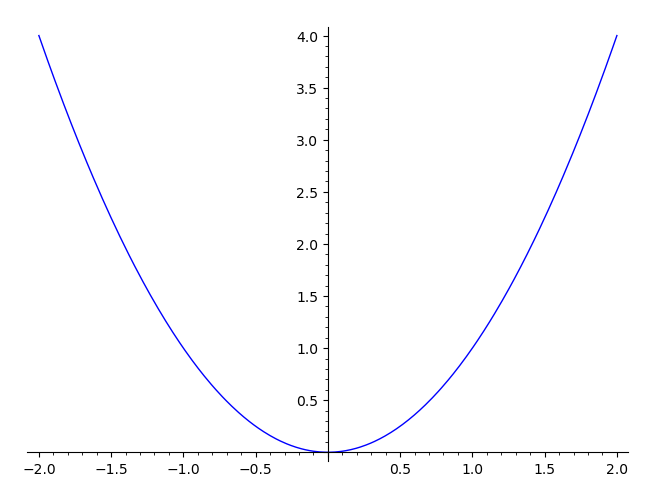
\includegraphics{parabola.png}
  Generally, a function $f: S\rightarrow T$ is given by a machine, formula or algorithm that
  computes $f(x)\in T$ for every $x\in S$. Nothing more, nothing less. It really has nothing to
  do with a graph (even though graphs can sometimes be useful for visualizing certain functions like $f(x) = x^2$).
\end{remark}


\begin{example}\label{crypthashex}
  Good examples of functions can be found in the \url{cryptographic hash functions}{https://en.wikipedia.org/wiki/Cryptographic_hash_function}. They are examples of complicated functions $f:S \rightarrow T$, where
  $S$ is infinite and $T$ finite. Here $S$ could be data like plain text files and $T$ could be
  a $256$ bit number. This is the setup for the widely used \texttt{sha-256} cryptographic hash function.
  The whole point of a cryptographic hash function is that it must be humanly impossible to
  \footnote{compute $y$ with $f(y) = f(x)$ given $f(x)$}{A pair $x\neq y$ with $f(x) = f(y)$ is called a collision}. 
  In fact, \texttt{sha-256} is used in the Bitcoin block chain. The precise definition of
  \texttt{sha-256} can be found in \url{FIPS PUB 180-4}{http://nvlpubs.nist.gov/nistpubs/FIPS/NIST.FIPS.180-4.pdf} approved by the Secretary of Commerce.

Other interesting functions output a bounded size digital footprint (checksum) of a file (like \url{\texttt{md5}}{https://en.wikipedia.org/wiki/MD5}). This is very useful
for checking data integrity of downloads over the internet. The \texttt{md5} hash is a $128$ bit number.

Instead of listing $256$ or $128$ bits for the hash value one uses hexadecimal notation with digits
in 0, 1, 2, 3, 4, 5, 6, 7, 8, 9 , a, b, c, d, e, f. A pair of hexadecimal digits then represents
a byte or $8$ bits. Output from \texttt{sha-256} and \texttt{md5} consist of $64$ and $32$ hexadecimal
digits respectively. You are welcome to experiment with these two hash functions in the
Sage window below.



\begin{sage}
import hashlib
print(hashlib.sha256(b"sha-256 is safe so far").hexdigest())
print(hashlib.md5(b"md5 has been broken").hexdigest())
\end{sage}

Another hashing function is \url{NeuralHash}{https://devpost.com/software/neuralhash} (see also \url{GitHub}{https://github.com/nikcheerla/neuralhash}) constructed using deep learning. It is used in Apple's Child
Sexual Abuse Material (\url{CSAM}{https://www.apple.com/child-safety/}) technology.
\end{example}


\beginshex
What is the \texttt{sha-256} hash of your name? Change a
few letters and recompute. Do you see any system? What about the \texttt{md5} hash function?
Can you find two different strings with the same \texttt{md5} hash using your computer?

\begin{hint}[showhide]
  I have not answered the last question myself, but I am told that it is possible to find
  a collision for \texttt{md5} using a garden variety home computer. Browsing the internet, it
  seems that the two strings $s_1$ and $s_2$ given in \footnote{hexadecimal notation}{This notation represents a sequence of bytes given by pairs of hexadecimal digits} by
\begin{code}
d131dd02c5e6eec4693d9a0698aff95c2fcab58712467eab4004583eb8fb7f89 
55ad340609f4b30283e488832571415a085125e8f7cdc99fd91dbdf280373c5b 
d8823e3156348f5bae6dacd436c919c6dd53e2b487da03fd02396306d248cda0 
e99f33420f577ee8ce54b67080a80d1ec69821bcb6a8839396f9652b6ff72a70
\end{code}
and
\begin{code}
d131dd02c5e6eec4693d9a0698aff95c2fcab50712467eab4004583eb8fb7f89 
55ad340609f4b30283e4888325f1415a085125e8f7cdc99fd91dbd7280373c5b 
d8823e3156348f5bae6dacd436c919c6dd53e23487da03fd02396306d248cda0 
e99f33420f577ee8ce54b67080280d1ec69821bcb6a8839396f965ab6ff72a70 
\end{code}
give a collision for \texttt{md5}. Verify that $s_1\neq s_2$ and
that they give the same \texttt{md5} hash. If you find a collision
for \texttt{sha-256} you will
become world famous.

\begin{hint}[showhide]
\begin{sage}
import hashlib
s1 = bytes.fromhex('d131dd02c5e6eec4693d9a0698aff95c2fcab58712467eab4004583eb8fb7f8955ad340609f4b30283e488832571415a085125e8f7cdc99fd91dbdf280373c5bd8823e3156348f5bae6dacd436c919c6dd53e2b487da03fd02396306d248cda0e99f33420f577ee8ce54b67080a80d1ec69821bcb6a8839396f9652b6ff72a70')
s2 = bytes.fromhex('d131dd02c5e6eec4693d9a0698aff95c2fcab50712467eab4004583eb8fb7f8955ad340609f4b30283e4888325f1415a085125e8f7cdc99fd91dbd7280373c5bd8823e3156348f5bae6dacd436c919c6dd53e23487da03fd02396306d248cda0e99f33420f577ee8ce54b67080280d1ec69821bcb6a8839396f965ab6ff72a70')
print(s1 == s2)
print(hashlib.md5(s1).hexdigest())
print(hashlib.md5(s2).hexdigest())
\end{sage}
\end{hint}
\end{hint}
\endshex

\subsection{Notations for defining a function}

If $f: S\rightarrow T$ is a function and $S$ is a finite set, then you can
define $f$ using a simple table. This is best illustrated using an
example. Suppose that $S = \{1, 2, 3\}, T = \RR$ and
\begin{align*}
  f(1) &= \sqrt{2}\\
  f(2) &= \pi\\
  f(3) &= -1.
\end{align*}
Then $f$ is expressed in table form as
$$
\def\arraystretch{1.5}
\begin{array}{c|ccccccc}
x & 1 & 2 & 3\\ \hline
f(x) & \sqrt{2} & \pi & -1
\end{array}
$$

Very often the bracket (or \emph{Tuborg} in Danish) notation is used. It is
similar to \texttt{if-then-else} statements in programming:
\begin{equation}\label{bracketsex}
f(x) =
\begin{cases}
  0 &\text{if } x\leq 0\\
  x^2 &\text{if } x > 0
\end{cases}
\end{equation}
defines the function $f:\RR \rightarrow \RR$ that outputs $0$ if the
input $x\leq 0$ and $x^2$ if $x>0$.


\beginshex
What is $f(-17)$ and $f(17)$ for the function defined in \eqref{bracketsex}. Draw
the graph of $f$. Come up with a function $f:S\rightarrow T$, where it
does not make sense to draw a graph.
\endshex


We now define three very important notions related to functions.

\begin{definition}[emph]
  Let $f: S\rightarrow T$ be a function. Then $f$ is called
  \begin{enumerate}[(i)]
  \item
    \emph{injective}, if $f(x) = f(y) \implies x = y$ for every $x, y\in S$.
  \item
    \emph{surjective}, if for every $y\in T$, there exists $x\in S$, such that $f(x) = y$.
  \item
    \emph{bijective}, if it is both injective and surjective.
  \end{enumerate}
\end{definition}

\beginshex
Is a cryptographic hash-function as defined in Example \ref{crypthashex} injective?
\endshex

\beginshex
Suppose that
$$
S = \{1, 2, 3\}\qquad\text{and}\qquad T = \{1, 2, 3, 4\}.
$$
We define a function $f: S\rightarrow T$ by the table
$$
\def\arraystretch{1.5}
\begin{array}{c|ccccccc}
x & 1 & 2 & 3\\ \hline
f(x) & 1 & 2 & 4
\end{array}
$$
Is $f$ injective? Is it surjective? Is it possible to adjust the table so that
$f$ becomes injective?
Is it possible to adjust the table so that
$f$ becomes surjective?
\endshex

\beginshex
Consider the function $f:S \rightarrow T$ given by
$$
f(x) = x^2,
$$
where $S = T = \RR$.
Is $f$ injective? Is $f$ surjective? Suggest how to change $S$ and $T$ so that $f:S\rightarrow T$ becomes
bijective.
\endshex

\beginshex
Consider the function $f:\ZZ \rightarrow \ZZ$ given by
$$
f(x) = x + 1
$$
Show that $f$ is bijective.
\endshex


\beginshex
Write down precisely how the truth table for $p\implies q$ may
be expressed in terms of a function $f: S\rightarrow T$. What are the sets $S$ and $T$ in this case?
\endshex


\subsection{Composition of functions}

Given two functions $f: S\rightarrow T$ and $g: U\rightarrow V$, where
$V\subseteq S$, we define a new function $f\circ g: U \rightarrow T$ by
$$
(f\circ g)(u) = f(g(u)).
$$
This notion calls for some reflection. We have a total of four sets
in this definition: $U, V, S$ and $T$ and, not to forget, the condition that
$V\subseteq S$. If this last condition was not satisfied it would be
meaningless to apply the function $f$ to $g(u)$.
I hope the diagram below helps the
understanding.

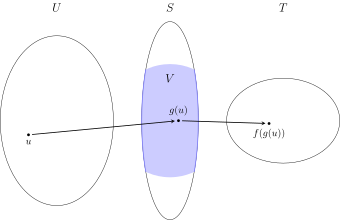
\includegraphics{compositefunction.svg}

\begin{remark}
  The concept of a function is powerful and underlies functional programming in computer science: every computation can be realized as applying a composition of functions to an argument. This is exemplified in the computer language
  \url{Haskell}{https://www.haskell.org/}.
  \end{remark}

\beginshex
Suppose that
$$
U = \{1, 2, 3\},\qquad S = \{1, 2, 3, 4\}\qquad\text{and}\qquad T = \{7, 8, 9\}
$$
and that $g: U \rightarrow S$ and $f: S\rightarrow T$ are given by the tables
$$
\def\arraystretch{1.5}
\begin{array}{c|ccccccc}
x & 1 & 2 & 3\\ \hline
g(x) & 1 & 3 & 4
\end{array}\qquad\text{and}\qquad
\begin{array}{c|ccccccc}
x & 1 & 2 & 3 & 4\\ \hline
f(x) & 7 & 8 & 9 & 7 
\end{array}
$$
Compute the table for $(f\circ g): U\rightarrow T$. Show that $f\circ g$ is not
injective. Adjust the table for $f$ so that $f\circ g$ becomes bijective.
\endshex

  
\beginshex
Consider $f: \RR\rightarrow \RR^2$ and $g: \RR^2\rightarrow \RR$ given by
\begin{align*}
  f(t) &= (t^2, t^3)\\
  g((x, y)) &= \cos(x y) + x \sin(x + y).
\end{align*}
What is $(g\circ f)(t)$ as a function from $\RR$ to $\RR$ in terms of $t$?
\endshex

\subsection{The inverse function}

If $f:S\rightarrow T$ is bijective, then we may define a function $g: T\rightarrow S$, so
that $(f\circ g)(y) = y$ for every $y\in T$ and $(g\circ f)(x)$ for every $x\in S$. This
function is denoted $f^{-1}$.

How do we define $f^{-1}(y)$ for $y\in T$? Well, since $f$ is surjective, we may find
$x\in S$ so that $y = f(x)$. Now, we simply define
\begin{equation}\label{invf}
f^{-1}(y) = x.
\end{equation}
We cannot have $x_1 \neq x_2$ in $S$ with $f(x_1) = f(x_2) = y$, since $f$ is injective. We only have one choice for
$x$ in \eqref{invf}. Therefore \eqref{invf} really is a good and sound definition.

\beginshex
Let $f: S\rightarrow S$, where $S = \{1, 2, 3\}$ be given by
$$
\def\arraystretch{1.5}
\begin{array}{c|ccccccc}
x & 1 & 2 & 3\\ \hline
f(x) & 3 & 1 & 2
\end{array}.
$$
Compute $f^{-1}$.

What if the definition of $f$ is changed to
$$
\def\arraystretch{1.5}
\begin{array}{c|ccccccc}
x & 1 & 2 & 3\\ \hline
f(x) & 3 & 2 & 2
\end{array}.
$$
Does $f^{-1}$ make sense here?
\endshex

\beginshex
What is the inverse function of $f:\ZZ\rightarrow \ZZ$ given by $f(x) = x + 1$?
What is the inverse function of $g: S \rightarrow S$, where $g(x) = \sqrt{x}$ and
$S = \{x\in \RR\mid x\geq 0\}$?
\endshex


\subsection{Neural networks}

Having defined functions and composition of functions, we can deflate
the term (deep) neural network, which is often clouded in
magic and mystery.

A \emph{neural network} is a special case of a function
\begin{equation}\label{neural}
f: A\rightarrow B,
\end{equation}
where $A\subseteq \RR^m$ and $B\subseteq \RR^n$. Neural networks are
often compositions of many intermediate functions called
(hidden) layers.


\begin{frameit}
A function such as \eqref{neural} can
be written
\begin{equation}\label{neuralfct}
f(x_1, \dots, x_m) = \left(
f_1(x_1, \dots, x_m), \dots, f_n(x_1, \dots, x_m)\right),
\end{equation}
where $f_1, \dots, f_n$ are functions $A\rightarrow \RR$.
\end{frameit}


In a neural
network the functions $f_1, f_2, \dots, f_n$ are viewed as neurons. Depending on their
input they either fire or do not fire a signal. Classically this is
modelled by the \url{perceptron}{https://en.wikipedia.org/wiki/Perceptron},
which is a function $p:\RR^n\rightarrow \RR$ of the form
\begin{equation}\label{relu}
p(x_1, \dots, x_n) =
\begin{cases}
  1 &\text{if } w_1 x_1 + \cdots + w_n x_n > b\\
  0 &\text{if } w_1 x_1 + \cdots + w_n x_n \leq b
\end{cases}
\end{equation}
  for fixed numbers $w_1, \dots, w_n$ (called weights) and a number $b$ (called the threshold).
  If the weighted sum $w_1 x_1 + \cdots + w_n x_n$ is above the threshold, the neuron
  fires (returns the value $1$). If not it does not fire (returns the value $0$).

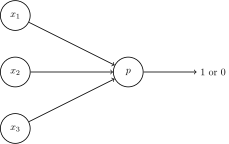
\includegraphics{perceptron.svg}


  \beginshex\label{perceptronex}
  Consider the three perceptrons $p_1, p_2, p_3: \RR^2\rightarrow \RR$, where
  $$
p_1(x, y) =
\begin{cases}
  1 &\text{if } -x-y > -\frac{3}{2}\\
  0 &\text{if } -x-y \leq -\frac{3}{2}
\end{cases},
\qquad
p_2(x, y) =
\begin{cases}
  1 &\text{if } x + y > \frac{1}{2}\\
  0 &\text{if } x + y \leq \frac{1}{2}
\end{cases},
$$
and
$$
p_3(x, y) =
\begin{cases}
  1 &\text{if } x + y > \frac{3}{2}\\
  0 &\text{if } x + y \leq \frac{3}{2}
\end{cases}.
$$
Let $f(x, y) = p_3 (p_1(x, y), p_2(x, y))$. Then $f$ is
a composite function $f = g\circ h$ of two functions $h: \RR^2\rightarrow \RR^2$
and $g: \RR^2\rightarrow \RR$. Write down these functions.

\begin{hideinbutton}{Hint}
Have a closer look at \eqref{neuralfct} in order to understand how
functions from $\RR^2$ to $\RR^2$ can written down.
\end{hideinbutton}

Compute
$f(0, 0), f(1, 0), f(0, 1)$ and $f(1, 1)$.



Relate the perceptrons $ p_1 $ and $ p_2 $ to the illustration
below. What do you think the red and blue line illustrate?  What does
it mean that a dot is solid compared to hollow? What is special
about points between the red and blue lines?  Try to relate $f(0,0),
f(1,0), f(0,1)$ and $f(1,1)$ to the illustration.

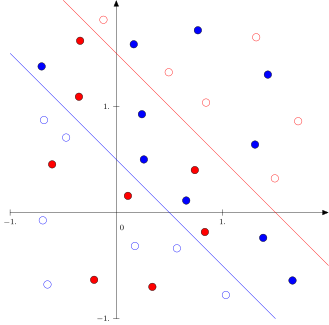
\includegraphics{whkperceptron.svg}

(Illustration courtesy of William Heyman Krill).

\endshex

  \beginshex
  Give weights $w_1, w_2$ and a threshold $b$ for a perceptron $p:\RR^2\rightarrow \RR$ that computes
  the logical and function $\land$ i.e, $p$ must satisfy
  \begin{align*}
    p(0,0) &= 0\\
    p(1, 0) &= 0\\
    p(0,1) &= 0\\
     p(1, 1) &= 1.
  \end{align*}
  Do the same for the logical or function $\lor$.
  \endshex
  
  The output of one neuron can be used as input for other neurons in a potentially extremely complicated network:

  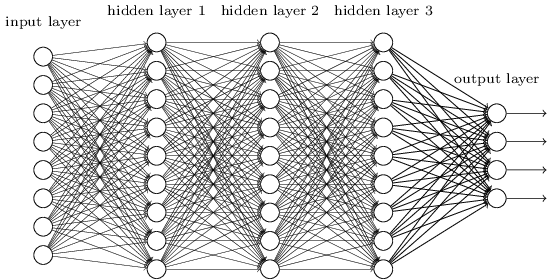
\includegraphics{deepneural.png}

  The diagram above represents a neural network, which is a function $\RR^8\rightarrow \RR^4$. This function
  is actually a composition (represented by the hidden layers $1$, $2$, $3$ and the output layer):
  $$
  \RR^8\rightarrow \RR^9 \rightarrow \RR^9 \rightarrow \RR^9 \rightarrow \RR^4.
  $$
  All of the nodes above, except the ones in the input layer, represent perceptrons.

  \beginshex 
  Is it possible to find a perceptron $p:\RR^2\rightarrow \RR$, such that
    \begin{align*}
    p(0,0) &= 0\\
    p(1, 0) &= 1\\
    p(0,1) &= 1\\
     p(1, 1) &= 0?
  \end{align*}
  What if you are allowed to use a neural network composed as $\RR^2\rightarrow \RR^2\rightarrow \RR$ (one hidden layer)
  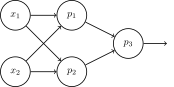
\includegraphics{xor.svg}?
  \endshex
  
  Mathematically there is no reason to use special functions such as perceptrons in each node. One also uses
  a (smooth) version of the perceptron employing the \url{sigmoid function}{https://en.wikipedia.org/wiki/Sigmoid_function}.
  With the notation above, this function is given as
  $$
  \sigma(x_1, \dots, x_n) = \frac{1}{1 + e^{-(w_1 x_1 + \cdots + w_n x_n) - b}}.
  $$
  However, around 2011 it was observed that the perceptron activation function (\url{ReLU}{https://en.wikipedia.org/wiki/Rectifier_(neural_networks)}) as defined in \eqref{relu} led to better training
  of deep neural networks. It is today, \url{the most popular activation function}{https://towardsdatascience.com/understanding-relu-the-most-popular-activation-function-in-5-minutes-459e3a2124f}.

\end{document}
